
% Simple LaTeX document example
\documentclass[11pt]{article}

% Include template

% Package imports and definitions
% (in alphabethical order)

% Used for color in text
% (Needed to be included early for some unknown dependency reason)
\usepackage[usenames,dvipsnames]{xcolor}

\usepackage{array}
\usepackage[english]{babel}
\usepackage{bytefield}
\usepackage{colortbl}
\usepackage{courier}
\usepackage{datetime}
\usepackage{enumitem}
\usepackage{eqparbox}
\usepackage{etoolbox}
\usepackage{fancyhdr}
\usepackage{float}

% Use T1 to get more font glyphs, e.g. to be able to write <>|
\usepackage[T1]{fontenc}

\usepackage[stable]{footmisc}
\usepackage{framed}

% Used for images and figures
\usepackage{graphicx}
\graphicspath{{./figures/}}
\graphicspath{{./}{./images/}}

\usepackage{grffile}

\usepackage[bookmarks, hidelinks]{hyperref}
\usepackage{hyperref}
% To get links in table of contents
\hypersetup{
  linktoc=all,
  hidelinks
}

\usepackage[utf8]{inputenc}
\usepackage{lastpage}

% Use lmodern to get searchable pdf
\usepackage{lmodern}

\usepackage{longtable}

\usepackage{ltablex}
% Using X keeps table width (default is max width)
\keepXColumns

\usepackage{mdframed}
\usepackage{microtype}
\usepackage{minibox}
\usepackage{pdflscape}
\usepackage{pdfpages}

% Silence some warnings
\usepackage{silence}
\WarningFilter{latex}{Underfull}
\WarningFilter{latex}{Overfull}
\WarningFilter{latex}{Text page}
\WarningFilter{pdfcolmk}{Nothing to fix}

\usepackage[usestackEOL]{stackengine}

% Used for side-by-side figures
\usepackage{subfig}

\usepackage{svg}
\usepackage{tabularx}
\usepackage{tcolorbox}
\usepackage{textcomp}
\usepackage{titlesec}
\usepackage{varioref}

% Add TikZ package for eg diagrams
\usepackage{tikz}
\usetikzlibrary{
    arrows.meta,
    positioning,
    shapes.geometric,
    automata
}

% Redefine auto-references
\def\paragraphautorefname{section}
\def\sectionautorefname{section}
\def\subsectionautorefname{section}
\def\subsubsectionautorefname{section}

% Set the page style
\pagestyle{fancy}

% Define custom colors
\definecolor{blue}{cmyk}{1,.50,0,.40}

% No indentation
\setlength{\parindent}          {0pt}

% Add some space between paragraphs
\setlength{\parskip}            {3pt plus 2pt}

% Set lenghts to use 16 pt usual spacing between lines
\setlength{\baselineskip}       {16.0pt}

% Margins
\setlength{\evensidemargin}     {0.5cm}
\setlength{\oddsidemargin}      {0.5cm}
\setlength{\marginparpush}      {1.0cm}
\setlength{\marginparsep}       {0.75cm}
\setlength{\marginparwidth}     {2.5cm}

\setlength{\textwidth}          {150mm}
\setlength{\headheight}         {29pt}

% Clear all header and footer fields
\fancyhf{}

% Set the left and right document header
\lhead
        {\eqparbox{maxColumnWidth}
            {\textcolor{Gray}
                {\scriptsize{Title}}\\
                 \scriptsize{My Document}
            }
        }
\chead
        {\eqparbox{maxColumnWidth}
            {\textcolor{Gray}
                {\scriptsize{Classification}}\\
                 \scriptsize{Public domain}
            }
        }
\rhead
        {\eqparbox{maxColumnWidth}
            {\textcolor{Gray}
                {\scriptsize{Version}}\\
                 \scriptsize{\ref{lastVersionNumber}}
            }
        }

% Redefine commands and formats for refs and dates
\renewcommand{\refname}{\section{References\protect}}
% Redefine date separator
\renewcommand{\dateseparator}{-}
% Redefine date format
\newdateformat{todaydate}{\THEYEAR-\twodigit{\THEMONTH}-\twodigit{\THEDAY}}
\todaydate

% Set the headruler width
\renewcommand{\headrulewidth}{1pt}
% Set the headruler color
\makeatletter
\renewcommand{\headrule}{
\setlength\@tempdima{\headrulewidth}
\textcolor{blue}{\hrule\@height\@tempdima\@width\headwidth}
\vskip -2\@tempdima}
\makeatother

% Title format
\titleformat{\paragraph}
{\normalfont\normalsize\bfseries}{\theparagraph}{1em}{}

\titlespacing*{\paragraph}
{0pt}{3.25ex plus 1ex minus .2ex}{1.5ex plus .2ex}

% subsubsub sections auto TOC entry
\setcounter{tocdepth}{4}

% Section numbering
\setcounter{secnumdepth}{4}


% Begin the document
\begin{document}

% Title page
\begin{titlepage}
    \begin{center}
        \vspace{0.3 cm}
        
\includegraphics[width=5cm]{figures/logo.jpg} \\
        \vspace{0.3 cm}
        \textcolor{blue}{{\Huge \textbf{My document}}} \\
        \vspace{0.4 cm}
        \textcolor{blue}{{\large Version: \ref{lastVersionNumber}}} \\
        \vspace{1.6 cm}
    \end{center}

    \begin{tcolorbox}[width=\textwidth, colframe={blue}, title=Classification: Public domain]
        This document and its contents \textbf{is fully free to use} and is in the public domain.\\
    \end{tcolorbox}

    \thispagestyle{empty}
    \hypersetup{pageanchor=false}
\end{titlepage}
\newpage

% Footer
\newpage
\fancyfoot[R]{Page \thepage\ of \pageref{LastPage}}

% Table of contents
\tableofcontents
\newpage

% Version list
\section{Version history}

\newcounter{version}

\begin{tabularx}{\textwidth}{
    |>{\centering\arraybackslash}p{1.2cm}
    |>{\centering\arraybackslash}p{2.2cm}
    |>{\centering\arraybackslash}p{3cm}
    |X|
}
    \hline
    \textbf{Version} &
    \textbf{Date} &
    \textbf{Author} &
    \textbf{Description} \\
    \hline
    \endfirsthead

    \hline
    \textbf{Version} &
    \textbf{Date} &
    \textbf{Author} &
    \textbf{Description} \\
    \hline
    \endhead

    \hline
    \multicolumn{4}{r}{\textit{Continued on next page}} \\
    \endfoot

    \hline
    \endlastfoot

    \refstepcounter{version}
    \theversion &
    2026-09-01 &
    Fredrik Hederstierna &
    First version made in \LaTeX. \\
    \hline

    \refstepcounter{version}
    \theversion &
    2026-09-10 &
    Fredrik Hederstierna &
    Renamed and updated. \newline
    Fixed. \\
    \hline

    \refstepcounter{version}
    \label{lastVersionNumber} % NOTE: keep this last to get version on title page and footer
    \theversion &
    2026-09-20 &
    Fredrik Hederstierna &
    \begin{itemize}[leftmargin=*, nosep]
    \item Renamed the project.
    \item Updated the architecture diagram.
    \item Corrected formatting.
    \end{itemize} \\

\end{tabularx}
\newpage

% Introduction
\section{Introduction}
This is the introduction.

% Enumeration style 'arabic' for numbers, 'Alph' for A-Z, 'alph' a-z, roman/Roman for ii/II,
% you can also add eg '.' or '()' around enum-char.
\begin{enumerate}[label=\textbf{\Roman*.}, ref=\Roman*]
    \setcounter{enumi}{0}
    \item First version made in \LaTeX.
    \item Changes.
    \begin{itemize}
        \item Renamed.
        \item Updated.
    \end{itemize}
    \item Corrected.
\end{enumerate}

\subsection{Subsection}
This is a subsection

\subsubsection{Subsubsection}
This is a subsubsection

% \setcounter{tocdepth}{4}
\paragraph{Subsubsubsection}
This is a subsubsubsection

\newpage

% Include stste diagram example
% Example of simple state machine using TikZ
\begin{figure}[ht]
    \centering

    \begin{tikzpicture}[
        ->,
        >=Stealth,
        node distance=3cm,
        every state/.style={thick}
    ]

    \node[state, initial] (idle) {Idle};
    \node[state, right=of idle] (active) {Active};
    \node[state, below=of active] (error) {Error};

    \path
        (idle) edge node[above] {start} (active)
        (active) edge[bend left] node[right] {fault} (error)
        (error) edge[bend left] node[left] {reset} (idle);

    \end{tikzpicture}

    \caption{System state machine.}
    \label{fig:state-machine}
\end{figure}


\newpage

% Include sequence diagram example
\begin{figure}[ht]
    \centering
    \includegraphics[width=0.85\textwidth]
        {figures/sequence_diagram.png}
    \caption{Sequence diagram example.}
    \label{fig:my-sequence-diagram}
\end{figure}

\newpage

% Include block diagram example
\begin{figure}[ht]
    \centering
    \includegraphics[width=0.85\textwidth]
        {figures/block_diagram.pdf}
    \caption{Block diagram example.}
    \label{fig:my-block-diagram}
\end{figure}

% End the document
\newpage
\end{document}
